\subsection{Bestimmung der Gegenspannung}
\label{sec:gegenspannung}
Um die Gegenspannung der einzelnen Spektrallinien zu bestimmen wird der Photostrom in Abhängigkeit einer angelegten Bremsspannung $U$ gemessen. Für jede der fünf ausgewerteten Spektrallinien werden zehn Messwerte im Bereich von  \num{-2} bis \num{2} Volt notiert.
Die hier betrachteten Spektrallinien der Quecksilberlampe sind:
\begin{align*}
	\text{rot:} \quad & \SI{615}{\nano\meter}
 \\
	\text{grün:} \quad & \SI{546}{\nano\meter}
 \\
	\text{lila:} \quad & \SI{435}{\nano\meter}
 \\
	\text{blau:} \quad & \SI{405}{\nano\meter}
 \\
	\text{UV:} \quad & \SI{365}{\nano\meter}
 \\
\end{align*}
Die gemessenen Daten sind in Tabelle \ref{tab:messdaten1}  zu sehen, in Tabelle \ref{tab:messdaten2} die Wurzel ihre gezogen und in Abbildung \ref{fig:spektrallinien} grafisch dargestellt. Wobei die Wurzel des Photostromes aufgetragen wird, um einen linearen Zusammenhang zu erhalten. Es gilt allgemein
\begin{align}
	I \sim U^2 \quad .
\end{align}

Deswegen wurden die negativen Photostöme nicht weiter beachtet, sodass zum Beispiel bei der roten Spektrallinie nur sechs von zehn Messwerten in der Auswertung berücksichtigt werden. \\
\begin{figure}[h!]
	\centering
	\captionof{table}{Gemessene Photoströme / \si{\pico\ampere}}
	\begin{tabular}{c|ccccc}
		Gegenspannung / V & rot & grün & lila & blau & UV \\
		\hline
		-2.00 & 8  & 260 & 600 & 350 & 360 \\
-1.60 & 6  & 240 & 520 & 280 & 300 \\
-1.20 & 6  & 200 & 400 & 250 & 270 \\
-0.80 & 4  & 140 & 310 & 200 & 230 \\
-0.40 & 2  & 90  & 220 & 140 & 160 \\
0.00  & 0  & 30  & 90  & 90  & 110 \\
0.40  & -1 & -20 & 50  & 38  & 66  \\
0.80  & -1 & -40 & 0   & 8   & 22  \\
1.20  & -1 & -40 & -4  & -2  & 4   \\
1.60  & -1 & -40 & -8  & -4  & -3  \\
2.00  & -1 & -40 & -10 & -5  & -5  \\

	\end{tabular}
	\label{tab:messdaten1}
\end{figure}

\begin{figure}[h!]
	\centering
	\captionof{table}{Wurzel der gemessene Photoströme / \si{\sqrt{\pico\ampere}}}
	\begin{tabular}{c|ccccc}
		Gegenspannung / V & rot & grün & lila & blau & UV \\
		\hline
	-2.00 & 2.8 & 16.1 & 24.5 & 18.7 & 19.0 \\
	-1.60 & 2.4 & 15.5 & 22.8 & 16.7 & 17.3 \\
	-1.20 & 2.4 & 14.1 & 20.0 & 15.8 & 16.4 \\
	-0.80 & 2.0 & 11.8 & 17.6 & 14.1 & 15.2 \\
	-0.40 & 1.4 & 9.5  & 14.8 & 11.8 & 12.6 \\
	0.00  & 0.0 & 5.5  & 9.5  & 9.5  & 10.5 \\
	0.40  & -- & --  & 7.1  & 6.2  & 8.1  \\
	0.80  & -- & -- & 0.0  & 2.8  & 4.7  \\
	1.20  & -- & --  & --  & --  & 2.0  \\
	1.60  & -- & --  & --  & --  & --  \\
	2.00  & -- & --  & -- & --  & --  \\
	\end{tabular}
	\label{tab:messdaten2}
\end{figure}

\begin{figure}[h!]
	\centering
	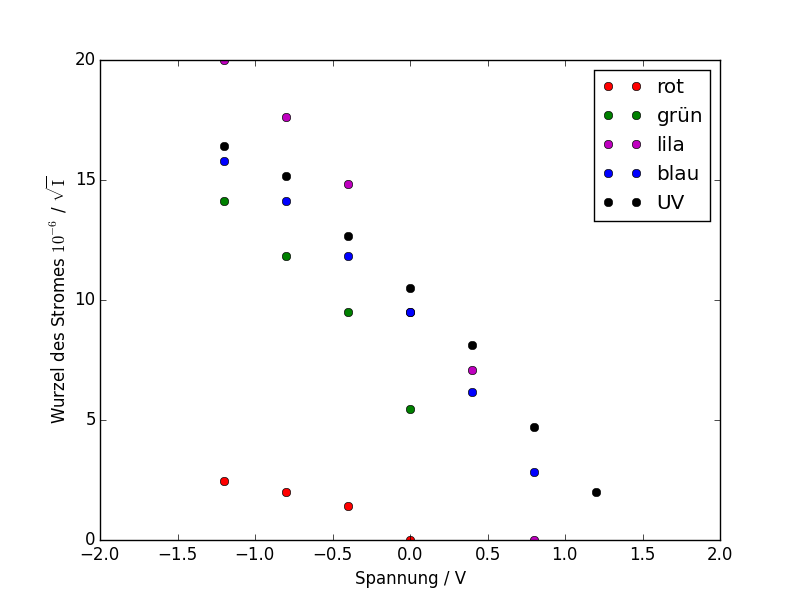
\includegraphics[width=\textwidth]{build/AlleWellenlangen.png}
	\caption{gemessene Spektrallinien}
	\label{fig:spektrallinien}
\end{figure}

\clearpage
Um die Grenzspannung $U_g$ zu bestimmen werden Ausgleichsgeraden mit Hilfe von Python nach den Formeln aus Kapitel \ref{sec:regression} erstellt und jeweils der x-Achsenabschnitt berechnet
\begin{align}
	\sqrt{I} = mU +b = 0\quad  \Leftrightarrow 	\quad U_g = - \frac{b}{m}
\end{align}	

Die Ausgleichsgeraden und Messwerte für jede Spektrallinie sind in den Abbildungen \ref{fig:regression_rot}, \ref{fig:regression_grun}, \ref{fig:regression_lila}, \ref{fig:regression_blau} und \ref{fig:regression_uv} dargestellt. Die berechneten Parameter sind

\begin{align*}
	\text{rot:} \quad m &= \SI{-0.00000126+-0.00000027}{\sqrt{\ampere}\per\volt}
 \\
	b &= \SI{0.00000059283+-0.00000033096}{}
 \\
	U_g &= \SI{0.46897+-0.28076}{\volt}
 \\[1em]
	\text{grün:} \quad m &= \SI{-0.00000525441+-0.00000068977}{\sqrt{\ampere}\per\volt}
 \\
	b &= \SI{6.0+-0.5}{\sqrt{\pico\ampere}}
 \\
	U_g &= \SI{1.30139+-0.23337}{}
 \\[1em]
	\text{lila:} \quad m &= \SI{-8.5+-0.7e-6}{\sqrt{\ampere}\per\volt}
 \\
	b &= \SI{0.00000945765+-0.00000072853}{\sqrt{\ampere}}
 \\
	U_g &= \SI{1.12+-0.12}{\volt}
 \\[1em]
	\text{blau:} \quad m &= \SI{-5.5+-0.4e-6}{\sqrt{\ampere}\per\volt}
 \\
	b &= \SI{8.7+-0.3}{\sqrt{\pico\ampere}}
 \\
	U_g &= \SI{1.3+-0.1}{\volt}
 \\[1em]
	\text{UV:} \quad m &= \SI{-0.00000529491+-0.00000034715}{\sqrt{\ampere}\per\volt}
 \\
	b &= \SI{9.6+-0.4e-6}{\sqrt{\ampere}}
 \\
	U_g &= \SI{1.82107+-0.13974}{}

\end{align*}












\begin{figure}[h!]
	\centering
	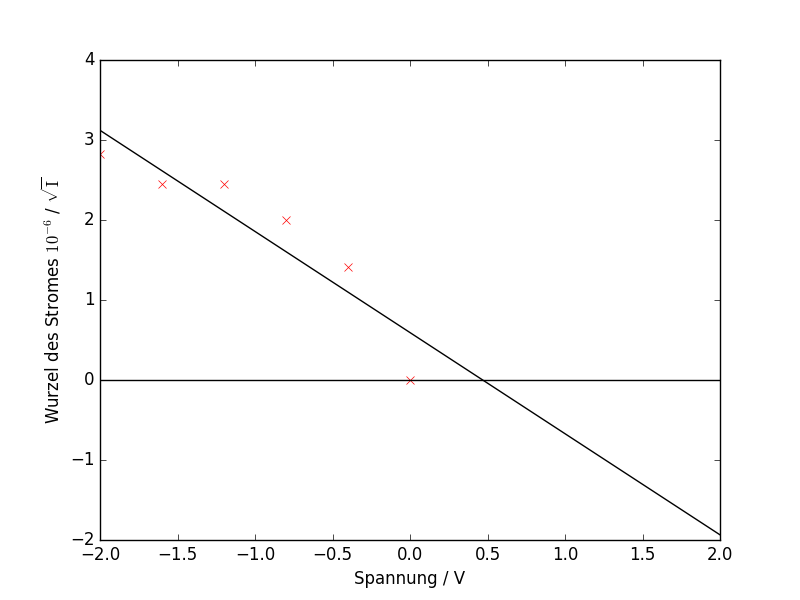
\includegraphics[width=0.8\textwidth]{build/regression_Farbe:0.png}
	\caption{Regression der roten Spektrallinie}
	\label{fig:regression_rot}
\end{figure}

\begin{figure}[h!]
	\centering
	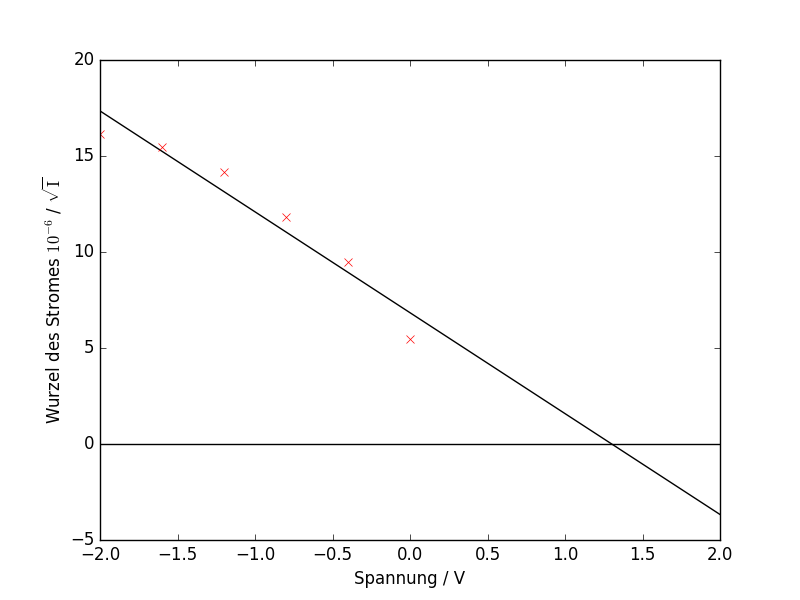
\includegraphics[width=0.8\textwidth]{build/regression_Farbe:1.png}
	\caption{Regression der grünen Spektrallinie}
	\label{fig:regression_grun}
\end{figure}

\begin{figure}[h!]
	\centering
	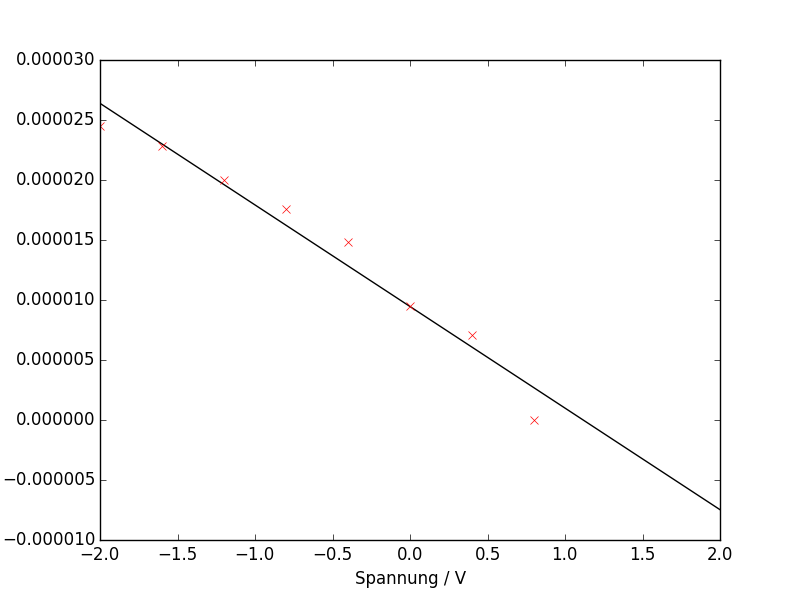
\includegraphics[width=0.8\textwidth]{build/regression_Farbe:2.png}
	\caption{Regression der lila Spektrallinie}
	\label{fig:regression_lila}
\end{figure}

\begin{figure}[h!]
	\centering
	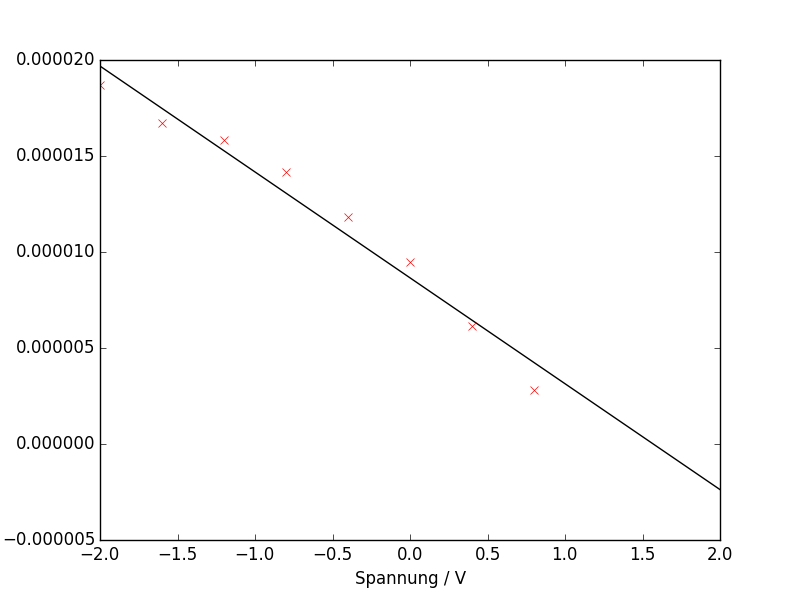
\includegraphics[width=0.8\textwidth]{build/regression_Farbe:3.png}
	\caption{Regression der blauen Spektrallinie}
	\label{fig:regression_blau}
\end{figure}

\begin{figure}[h!]
	\centering
	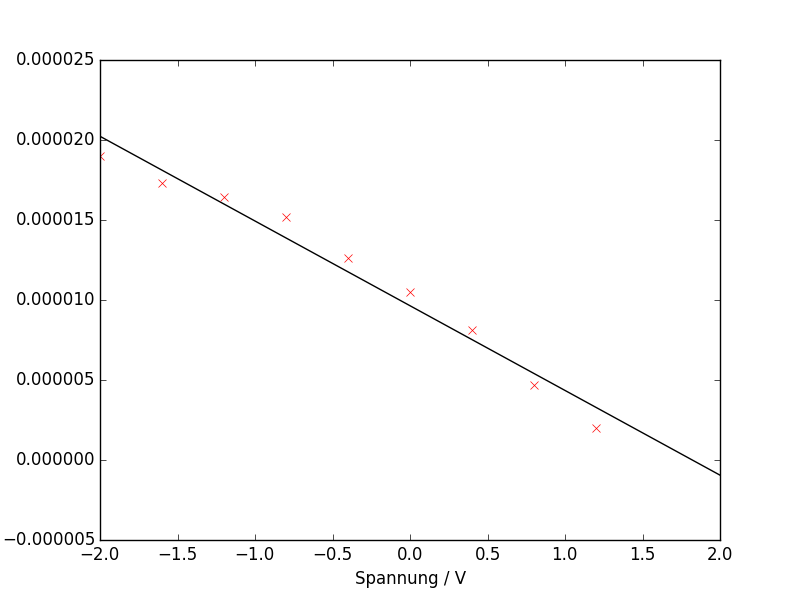
\includegraphics[width=0.8\textwidth]{build/regression_Farbe:4.png}
	\caption{Regression der ultravioletten Spektrallinie}
	\label{fig:regression_uv}
\end{figure}

\begin{figure}[h!]
\centering
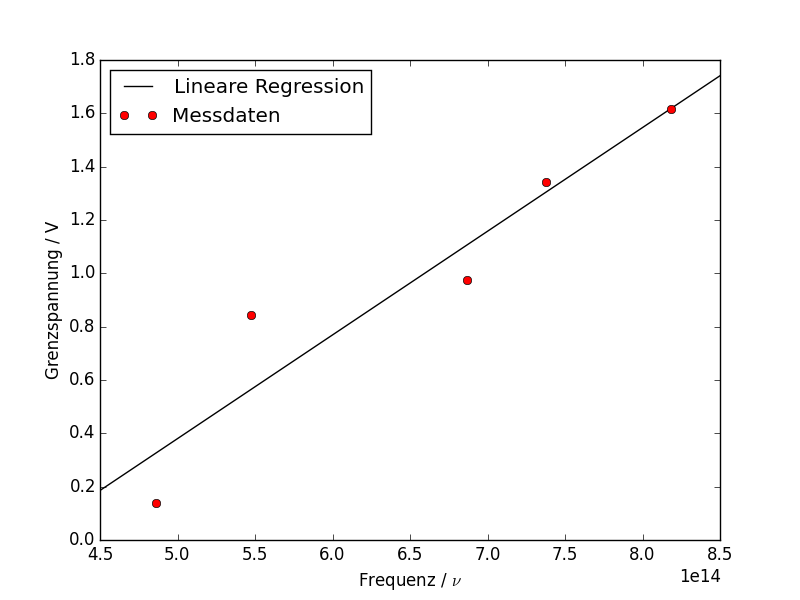
\includegraphics[width=0.8\textwidth]{build/regression_aufgabe2.png}
\caption{Regression zur Bestimmung von $h$ und $A_k$}
\label{fig:regression2}
\end{figure}


\clearpage

\subsection{Bestimmung des Verhältnisses $\frac{h}{e_0}$}
\label{sec:h_durch_h}
Die Gleichungen \eqref{eq:Energie} und \eqref{eq:einstein} liefern beide einen Ausdruck für die Energie der Photoelektronen. Durch Gleichsetzen ergibt sich
\begin{align}
	h\nu = e_0U_g \ .
\end{align}
Da nach dem vorigen Kapitel die Gegenspannungen bekannt sind, kann mit Hilfe einer linearen Regression das Verhältnis vom Planckschen Wirkungsquantum $h$ zur Elementarladung $e_0$ bestimmt werden. Auch die Austrittsarbeit $A_k$ kann auf diese Weise bestimmt werden.
\begin{align}
	U_g = -\frac{A_k}{e_0} +\nu \frac{h}{e_0} = b + m \cdot \nu
\end{align}
Die Wellenlänge des Lichtes  wird zunächst in die Frequenz umgerechnet
\begin{align}
	\nu = \frac{c}{ \lambda}, \quad c =\SI{298792458}{\meter\per\second} \quad .
\end{align}
Die Werte sind in Tabelle \ref{tab:h_durch_e} aufgetragen.
\begin{figure}[h!]
	\centering
	\captionof{table}{Gemessene Photoströme / \si{\pico\ampere}}
	\begin{tabular}{c|c|c}
		Gegenspannung / V & Wellenlange / \si{\nano\meter}  & Frequenz / \si{\tera\hertz}\\
		\hline
		0.47 & 615 & 486 \\
1.30 & 546 & 547 \\
1.12 & 435 & 687 \\
1.57 & 405 & 738 \\
1.82 & 365 & 819 \\

	\end{tabular}
	\label{tab:h_durch_e}
\end{figure}

Die lineare Regression liefert schlussendlich den Graph, der in Abbildung \ref{fig:regression2} dargestellt ist und folgende Werte:



\begin{align}
	& m = \frac{h}{e_0} = \SI{3.89+-0.77e-15}{\volt\second}
 \\
	& \Rightarrow h =  \SI{3.2+-1.1e-15}{\electronvolt\second}
 \\
	& b = - \frac{A_k}{e_0} = \SI{-0.86+-0.74}{\volt}
 \\
	& \Rightarrow A_k = \SI{1.56+-0.51}{\electronvolt}
 \label{eq:austrittsarbeit}
	\end{align}
	
	
\clearpage
\subsection{Photostrom des orangenen Spektrallinie}
Bei der orangenen Spektralline ($\lambda = \SI{578}{\nano\meter}$) wird der Photonenstrom wie bei den anderen Spektrallinen auch gemessen - hier aber über eine größeres Intervall der Bremsspannung von  \num{-20} bis \num{20} Volt. Die Daten (siehe Tabelle \ref{tab:orange}) werden aufgetragen und der in Abbildung \ref{fig:orange} dargestellte Plot beschrieben. \\
Für hohe beschleunigende Spannungen -- d.h. niedrige Bremsspannung -- erreicht der Photonenstrom einen Grenzwert. Das liegt daran, dass nicht beliebig viele Elektronen zur Verfügung stehen, sonder nur so viele, wie durch die Lichtquelle aus der Elektronenkathode ausgelöst werden. Das heißt, dass die Intensität der Lichtquelle den Grenzwert des Photonenstromes bestimmt. \\
Dieser Grenzwert wird mit der vorliegenden Versuchsanordnung allerdings nie erreicht werden. Nicht alle freiwerdenden Elektronen erreichen die Anode, da ihre Kapazität beschränkt ist. Eine Verbesserung  im Versuchsaufbau, um möglichst nah an den Grenzwert zu kommen, ist eine größere Anode. \\

Der Photostrom bricht nicht abrupt auf null ab, wenn die Grenzspannung erreicht ist. Die Elektronen haben bereits in dem Material eine Energie (Fermi-Energie), die in Abhängigkeit von den Elektronenkonfigurationen variiert. Obwohl alle Elektronen die gleiche Lichtintensität erfahren, werden deswegen einige Elektronen die Anode bereits erreichen, währen andere nicht über die hinreichende Energie verfügen. \\
Für hinreichend große Bremsspannungen tritt ein negativer Photonenstrom auf. Wegen der niedrigen Verdampfungstemperatur der Kathode, wird schon bei Raumtemperatur Material der Kathode freigesetzt, dass sich auf der Anode ansammelt. Als Folge tritt ein Photoeffekt an der Anode auf : Es werden Elektronen freigesetzt, die zu einem negativen Strom führen.

\begin{figure}[h!]
	\centering
	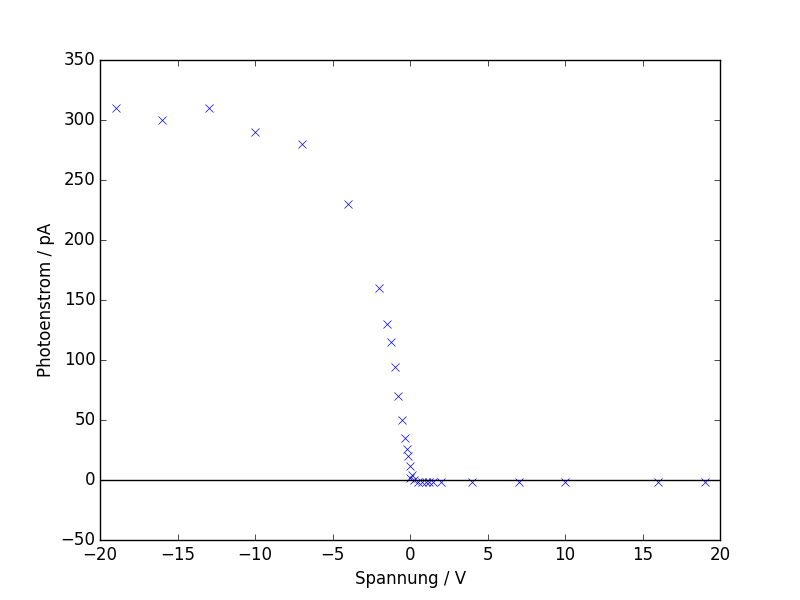
\includegraphics[width=\textwidth]{build/OrangeWellenlange.png}
	\caption{Photonenstrom der $\lambda = 578 \si{\nano\meter}$ Spektrallinie}
	\label{fig:orange}
\end{figure}

\begin{figure}[h!]
	\centering
	\captionof{table}{Gemessenen Photostrom der $\lambda = 578 \si{\nano\meter}$ Spektrallinie}
	\begin{tabular}{c|c}
		Gegenspannung / V & Photostrom / \si{\pico\ampere}  \\
		\hline
		19.00  & -2  \\
16.00  & -2  \\
10.00  & -2  \\
7.00   & -2  \\
4.00   & -2  \\
2.00   & -2  \\
1.50   & -2  \\
1.25   & -2  \\
1.00   & -2  \\
0.75   & -2  \\
0.50   & -2  \\
0.25   & 0   \\
0.02   & 2   \\
0.10   & 4   \\
0.00   & 12  \\
-0.10  & 20  \\
-0.20  & 26  \\
-0.30  & 35  \\
-0.50  & 50  \\
-0.75  & 70  \\
-1.00  & 94  \\
-1.25  & 115 \\
-1.50  & 130 \\
-2.00  & 160 \\
-4.00  & 230 \\
-7.00  & 280 \\
-10.00 & 290 \\
-13.00 & 310 \\
-16.00 & 300 \\
-19.00 & 310 \\

	\end{tabular}
	\label{tab:orange}
\end{figure}

	
